\chapter{Qualidade de Energia em Aeronaves}
\todo[inline]{30 P�gs}

O mercado da avia��o tem passado por uma mudan�a nos preceitos de desenvolvimento de sistemas que v�o desde a utiliza��o de novas tecnologias embarcadas at� a mudan�a na concep��o de opera��o da aeronave. Essa tend�ncia vem ocorrendo de maneira natural como evolu��o do mercado pela demanda de aeronaves mais eficientes e competitivas. Nesse contexto h� o conceito de \textit{More Electric Aircraft} (MEA). Como o pr�prio nome diz, essa concep��o baseia-se em aeronaves cuja filosofia de projeto contempla o uso abundante de sistemas alimentados eletricamente com o objetivo de aumentar a efici�ncia.\todo[inline]{D� de encher mais lingui�a pelas referencias Abdelhafez2009} Isso pode ser visto nos mais recentes desenvolvimentos de aeronaves, como por exemplo o Boeing 787, onde a redu��o da emiss�o de CO\textsubscript{2} � 20\% menor se comparado com o Boeing 767. \cite{Boeing2007}. O ganho n�o se d� apenas na redu��o do consumo de combust�vel e emiss�o de gases pela queima de combust�veis f�sseis, mas h� tamb�m a redu��o de peso e volume de sistemas, aumento de seguran�a, melhora na confiabilidade e manutenabilidade \cite{Boeing2007,Abdelhafez2009}.

Nesse contexto, a gera��o de energia el�trica 

Assim, o uso de conversores para alimentar cargas nao lineares vem poluindo a rede

o uso de cargas nao lineares suja a rede, degradando a qualidade de energia

os problemas da energia suja s�o 

metodos s�o necess�rios para mitigar esse problema

\begin{figure}[ht]
	\centering
	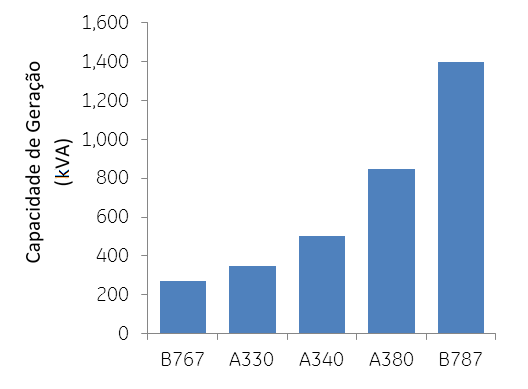
\includegraphics[width=0.7\textwidth]{Cap2/Figuras/trend.png}
	\caption{\cite{Frost2008}}
	\label{fig:trend.png}
\end{figure}

\begin{figure}[ht]
	\centering
	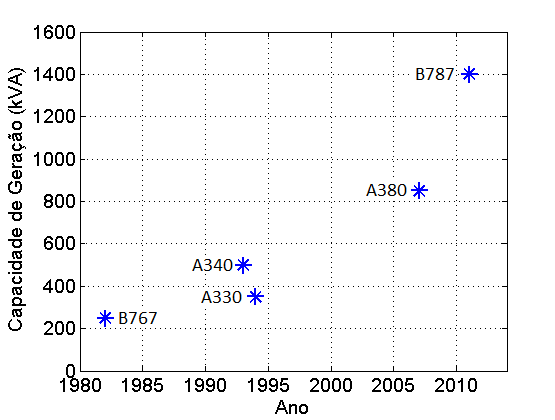
\includegraphics[width=0.7\textwidth]{Cap2/Figuras/trend_year.png}
	\caption{trend }
	\label{fig:trend_year.png}
\end{figure}

\section{Conversores com Alto Fator de Pot�ncia}

\section{Filtros Passivos}

\section{Filtros Ativos}




